

\begin{center}
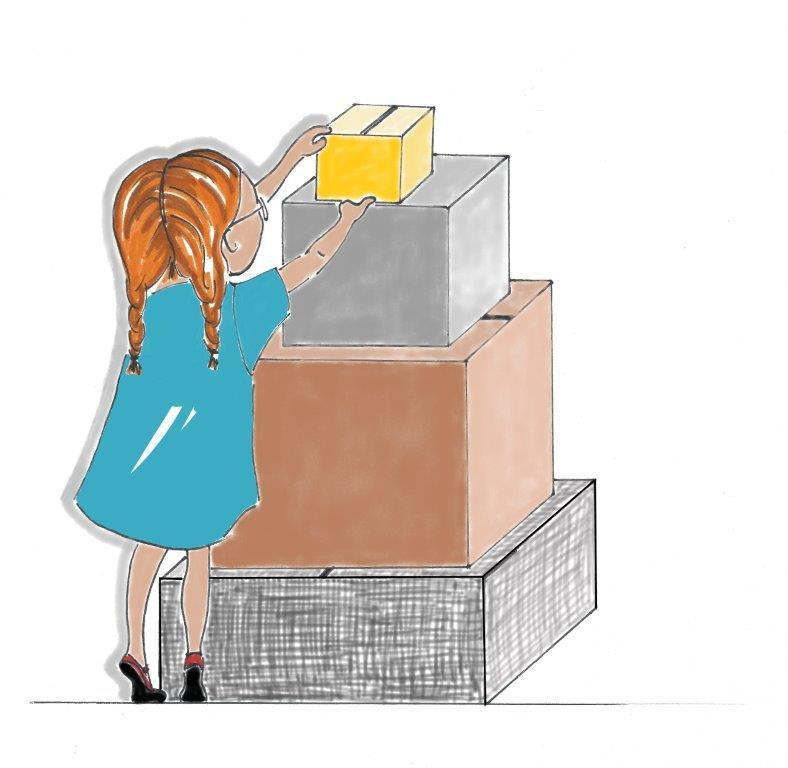
\includegraphics[width=0.6\textwidth]{content/3/chapter4/images/11.png}\\
Cippi在准备包裹
\end{center}

模块是C++20的四大特性之一,模块的功能有很多:更短的编译时间,隔离宏,取消头文件,避免丑陋的工作区。在介绍模块的优点之前,先来一起了解一下模块。

\subsubsubsection{4.2.1\hspace{0.2cm}为什么需要模块?}

从一个简单的可执行文件开始,我创建了一个helloWorld.cpp程序。

\hspace*{\fill} \\ %插入空行
\noindent
\textbf{一个简单的hello world程序}
\begin{lstlisting}[style=styleCXX]
// helloWorld.cpp

#include <iostream>

int main() {
	std::cout << "Hello World" << '\n';
}
\end{lstlisting}

使用\href{http://gcc.gnu.org/}{GCC}可将helloWorld.cpp编译成一个可执行的helloWorld,可执行文件的大小是文本文件的130倍。

\begin{center}
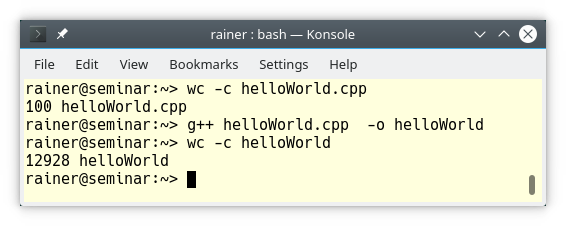
\includegraphics[width=0.8\textwidth]{content/3/chapter4/images/12.png}\\
目标文件的大小
\end{center}

截图中的数字100和12928代表字节数。现在,我们再对底层发生的事情进行一下了解。

\hspace*{\fill} \\ %插入空行
\noindent
\textbf{4.2.1.1\hspace{0.2cm}传统的构建过程}

构建过程包括三个步骤:预处理、编译和链接。

\hspace*{\fill} \\ %插入空行
\noindent
\textbf{4.2.1.1.1\hspace{0.2cm}预处理}

预处理器以\#include和\#define的方式处理指令。预处理器用相应的头文件替换\#include指令,并替换宏(\#define)。因为诸如\#if,\#else,\#elif,\#ifdef,\#ifndef和\#endif等指令,源代码的一部分可以包含或排除。

这个简单的文本替换过程(宏展开)可以通过在GCC/Clang上使用编译器标志-E,或在Windows上使用/E,就可以进行查看了。

\begin{center}
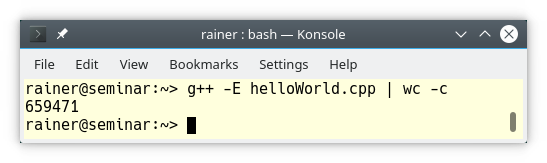
\includegraphics[width=0.8\textwidth]{content/3/chapter4/images/13.png}\\
预处理器的输出
\end{center}

哇! !预处理步骤的输出超过50万个字节。我不想责怪GCC,其他编译器也同样啰嗦。预处理器的输出则是编译器的输入。

这个预处理步骤的结果就是翻译单元。

\hspace*{\fill} \\ %插入空行
\noindent
\textbf{4.2.1.1.2\hspace{0.2cm}编译}

在预处理器的输出上分别执行编译,编译器解析C++源代码,并将其转换为汇编代码。生成的文件称为目标文件,包含二进制形式的编译代码。目标文件可以引用没有定义的符号,也可以放在存档文件中以供以后重用。这些存档文件称为静态库。

编译器生成的对象文件则是链接器的输入。

\hspace*{\fill} \\ %插入空行
\noindent
\textbf{4.2.1.1.3\hspace{0.2cm}连接}

链接器的输出可以是可执行库、静态库或动态库。链接器的工作是解析对未定义符号的引用,符号在目标文件或库中定义。这个阶段常见的错误是符号没有定义或者定义了不止一次。

这个由三个步骤组成的构建过程继承自C。若只有一个翻译单元,就能很好地工作。但若有不止一个翻译单元,就会出现很多问题。

\hspace*{\fill} \\ %插入空行
\noindent
\textbf{4.2.1.2\hspace{0.2cm}构建中的问题}

下面是经典构建过程中缺陷的不完整列表,这些缺陷可以通过模块来解决。

\hspace*{\fill} \\ %插入空行
\noindent
\textbf{4.2.1.2.1\hspace{0.2cm}重复替换}

预处理器用相应的头文件替换\#include指令。修改一下helloWorld.cpp程序,使重复可见。我重构了程序并添加了两个源文件hello.cpp和world.cpp。源文件hello.cpp提供了hello函数,源文件world.cpp提供了world函数。

两个源文件都包含相应的头文件。重构意味着具有与前面的程序helloWorld.cpp相同的外部行为,但内部结构进行了改进。以下是新文件:

\begin{itemize}
\item 
hello.cpp和hello.h

\noindent
hello的实现
\begin{lstlisting}[style=styleCXX]
// hello.cpp

#include "hello.h"

void hello() {
	std::cout << "hello ";
}
\end{lstlisting}

\noindent
hello的头文件
\begin{lstlisting}[style=styleCXX]
// hello.h

#include <iostream>

void hello();
\end{lstlisting}

\item 
world.cpp和world.h

\noindent
world的实现
\begin{lstlisting}[style=styleCXX]
// world.cpp

#include "world.h"

void world() {
	std::cout << "world";
}
\end{lstlisting}

\noindent
world的头文件
\begin{lstlisting}[style=styleCXX]
// world.h

#include <iostream>

void world();
\end{lstlisting}

\item 
helloWorld2.cpp

\noindent
使用hello和world
\begin{lstlisting}[style=styleCXX]
// helloWorld2.cpp

#include <iostream>

#include "hello.h"
#include "world.h"

int main() {
	
	hello();
	world();
	std::cout << '\n';
}
\end{lstlisting}


\end{itemize}

构建和执行如预期的一样:

\begin{center}
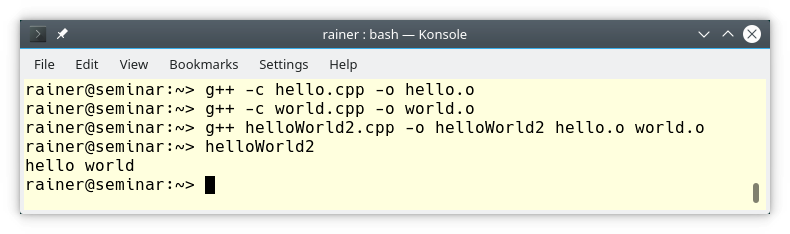
\includegraphics[width=0.8\textwidth]{content/3/chapter4/images/14.png}\\
编译的一个简单程序
\end{center}

问题是这样的。预处理器运行在每个源文件上,所以头文件<iostream>总共包含了三次。因此,每个源文件均多了50多万行代码。

\begin{center}
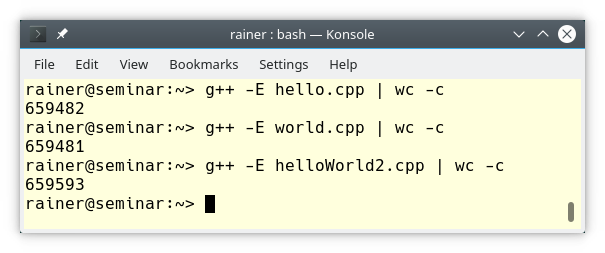
\includegraphics[width=0.8\textwidth]{content/3/chapter4/images/15.png}\\
预处理源文件的大小
\end{center}

这是对编译时间的浪费。

与头文件不同,模块只导入一次,而且不会有什么开销。

\hspace*{\fill} \\ %插入空行
\noindent
\textbf{4.2.1.2.2\hspace{0.2cm}隔离预处理宏}

若C++社区有一个共识的话,那就是:应该去掉预处理器宏。为什么?使用宏只是简单的文本替换,不包括任何C++语义。当然,这有许多负面后果:例如,这可能取决于包含宏的顺序,或者宏可能与应用程序中已经定义的宏或名称冲突。

假设有两个头文件webcolors.h和productininfo.h。

\hspace*{\fill} \\ %插入空行
\noindent
\textbf{先定义一个宏RED}
\begin{lstlisting}[style=styleCXX]
// webcolors.h
#define RED 0xFF0000
\end{lstlisting}

\noindent
\textbf{再定义一个宏RED}
\begin{lstlisting}[style=styleCXX]
// productinfo.h
#define RED 0
\end{lstlisting}

当源文件client.cpp包含两个头文件时,宏RED的值取决于所包含头文件的顺序。这种依赖关系非常容易出错。

模块则没有导入顺序的问题。

\hspace*{\fill} \\ %插入空行
\noindent
\textbf{4.2.1.2.3\hspace{0.2cm}隔离宏}

ODR代表单一定义规则,对于函数:

\begin{itemize}
\item 
函数在任何翻译单元中不能有一个以上的定义。

\item 
函数在程序中不能有多个定义。
\end{itemize}

可以在多个翻译单元中定义具有外部链接的内联函数,而宏必须满足每个定义的要求。

当链接一个违背单一定义规则的程序时,链接器会怎么样。下面的代码示例有两个头文件,header.h和header2.h。主程序包含头文件header.h两次,因此,由于包含了func的两个定义,因此违背了单一定义规则。

\hspace*{\fill} \\ %插入空行
\noindent
\textbf{函数func的定义}
\begin{lstlisting}[style=styleCXX]
// header.h
void func() {}
\end{lstlisting}

\noindent
\textbf{将函数定义间接包含到func中}
\begin{lstlisting}[style=styleCXX]
// header2.h
#include "header.h"
\end{lstlisting}

\noindent
\textbf{双重定义的函数func}
\begin{lstlisting}[style=styleCXX]
// main.cpp

#include "header.h"
#include "header2.h"

int main() {}
\end{lstlisting}

链接器会说,func有多个定义:

\begin{center}
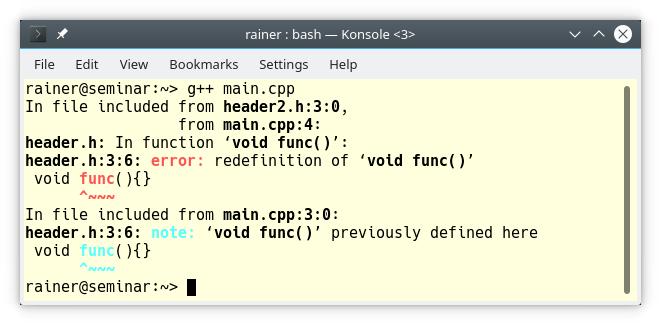
\includegraphics[width=0.8\textwidth]{content/3/chapter4/images/16.png}\\
违背了单一定义规则
\end{center}

我们已经习惯了一些丑陋的方法,比如在头文件周围加一个包含守卫。在头文件header.h中添加包含守卫FUNC\_H可以解决这个问题。

\hspace*{\fill} \\ %插入空行
\noindent
\textbf{使用包含守卫来解决ODR问题}
\begin{lstlisting}[style=styleCXX]
// header.h

#ifndef FUNC_H
#define FUNC_H

void func(){}

#endif
\end{lstlisting}

对于模块,不太可能出现重复符号。

那么,现在我将来说说模块的优势。

\subsubsubsection{4.2.2\hspace{0.2cm}优势}

下面以简洁的形式介绍模块的优势:

\begin{itemize}
\item 
模块只导入一次,而且实际上编译开销很小。

\item 
导入模块没有顺序之分。

\item 
模块不可能重复符号。

\item 
模块能够表达代码的逻辑结构。可以显式地指定应导出或不应导出的名称,还可以将几个模块捆绑到一个更大的模块中,并将它们作为逻辑包提供出去。

\item 
由于模块,不需要再将源代码分离为接口和实现部分。
\end{itemize}

\begin{tcolorbox}[breakable,enhanced jigsaw,colback=blue!5!white,colframe=blue!75!black,title=常规类型]
C++中的模块可能比你想象的要更加古老。简短的历史回顾应该能让你了解,把如此有价值的东西纳入C++标准需要多长时间。

\hspace*{\fill} \\ %插入空行
2004年,Daveed Vandevoorde写了一份提案\href{http://www.open-std.org/jtc1/sc22/wg21/docs/papers/2004/n1736.pdf}{N1736.pdf},第一次描述了模块的思想。不过,直到2012年才成立了专门的研究小组(SG2,模块)。2017年,Clang 5.0和MSVC 19.1提供了第一个实现。一年后,模块TS(技术规范)确定。大约在同一时间,Google针对模块提出了所谓的ATOM(Another Take On Modules)提案(\href{http://www.open-std.org/jtc1/sc22/wg21/docs/papers/2018/p0947r1.html}{P0947})。2019年,Modules TS和ATOM提案合并到C++20委员会草案中(\href{https://github.com/cplusplus/draft/releases/tag/n4842}{N4842})。
\end{tcolorbox}

\subsubsubsection{4.2.3\hspace{0.2cm}一个例子}

本节的目的很简单:向您介绍模块。模块的更高级特性将在后面几节中介绍。让我们从一个简单的数学模块开始吧。

\hspace*{\fill} \\ %插入空行
\noindent
\textbf{简单的math模块}
\begin{lstlisting}[style=styleCXX]
// math.ixx

export module math;

export int add(int fir, int sec){
	return fir + sec;
}
\end{lstlisting}

表达式导出模块math是模块声明。通过将export放在函数add的定义之前,add导出,因此模块的使用者可以使用。

\hspace*{\fill} \\ %插入空行
\noindent
\textbf{使用math模块}
\begin{lstlisting}[style=styleCXX]
// client.cpp

import math;

int main() {
	add(2000, 20);
}
\end{lstlisting}

import math导入math模块,并使模块中导出的名称对client.cpp可见。

让我们从模块声明文件开始。

\hspace*{\fill} \\ %插入空行
\noindent
\textbf{4.2.3.1\hspace{0.2cm}模块的声明文件}

是否注意到模块的奇怪名称:math.ixx。

\begin{itemize}
\item 
Microsoft编译器使用扩展名ixx。后缀ixx代表模块接口源。

\item 
Clang编译器最初使用扩展cppm,后缀中的m可能代表模块。这个约定在Clang的新版本中更改为cpp扩展。

\item 
GCC编译器则不使用特殊的扩展。
\end{itemize}

全局模块用于组合模块接口,以关键字module开始,以模块声明结束。全局模块可以出现在使用预处理器指令(如\#include)的地方,以便模块接口可以编译。全局模块片段中的代码,不会由模块接口导出。

math模块的第二个版本支持add和getProduct两个函数。

\hspace*{\fill} \\ %插入空行
\noindent
\textbf{全局模块的定义}
\begin{lstlisting}[style=styleCXX]
// math1.ixx

module;

#include <numeric>
#include <vector>

export module math;

export int add(int fir, int sec){
	return fir + sec;
}

export int getProduct(const std::vector<int>& vec) {
	return std::accumulate(vec.begin(), vec.end(), 1, std::multiplies<int>());
}
\end{lstlisting}

我在全局模块(第3行)和模块声明(第8行)之间包含了必要的头文件。

\hspace*{\fill} \\ %插入空行
\noindent
\textbf{使用改进的math模块}
\begin{lstlisting}[style=styleCXX]
// client1.cpp

#include <iostream>
#include <vector>

import math;

int main() {
	
	std::cout << '\n';
	
	std::cout << "add(2000, 20): " << add(2000, 20) << '\n';
	
	std::vector<int> myVec{1, 2, 3, 4, 5, 6, 7, 8, 9, 10};
	
	std::cout << "getProduct(myVec): " << getProduct(myVec) << '\n';
	
	std::cout << '\n';
}
\end{lstlisting}

客户端导入math模块,并使用它的功能:

\begin{center}
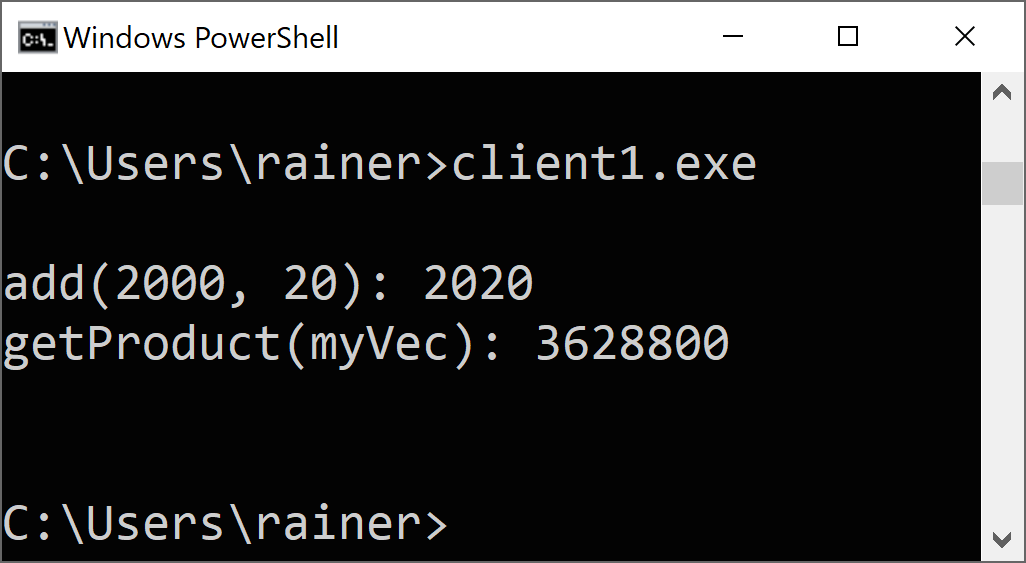
\includegraphics[width=0.5\textwidth]{content/3/chapter4/images/17.png}\\
执行程序client1.exe
\end{center}

现在,让我们深入的了解一下细节。

\subsubsubsection{4.2.4\hspace{0.2cm}编译和使用}

编译math模块。若客户端程序client.cpp使用ixx,则必须使用最新的Clang、GCC或Microsoft编译器。

模块的编译还是具有挑战性。因此,我将用Microsoft编译器和Clang编译器作为示例来演示模块的编译。

\hspace*{\fill} \\ %插入空行
\noindent
\textbf{4.2.4.1\hspace{0.2cm} Microsoft Visual编译器}

首先,我使用cl.exe 19.25.28614(x64)编译器。

\begin{center}
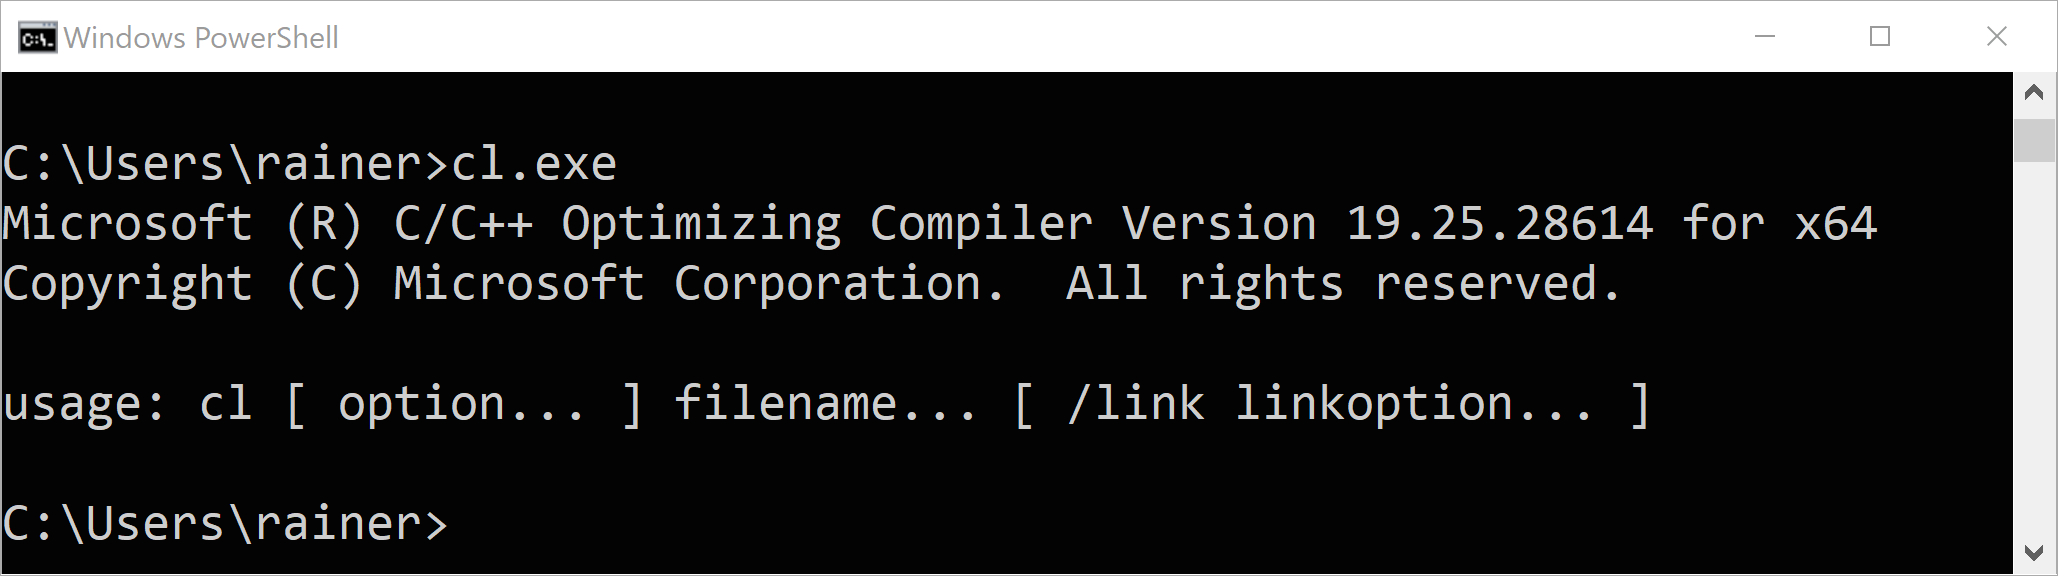
\includegraphics[width=0.8\textwidth]{content/3/chapter4/images/18.png}\\
Microsoft的编译器
\end{center}

这些是使用Microsoft编译器编译和使用模块的步骤,我只展示了最短的命令行示例。如承诺的,更多细节将随之而来。此外,对于旧的微软编译器,必须使用/std:cpplatest编译标志。

\hspace*{\fill} \\ %插入空行
\noindent
\textbf{使用Microsoft编译器构建可执行文件}
\begin{tcblisting}{commandshell={}}
cl.exe /experimental:module /c math.ixx
cl.exe /experimental:module client.cpp math.obj
\end{tcblisting}

\begin{itemize}
\item 
第1行创建一个目标文件math.obj和一个IFC文件math.ifc。IFC文件包含模块接口的元数据描述。IFC的二进制格式是模仿Gabriel Dos Reis和Bjarne Stroustrup(2004/2005)的\href{https://www.stroustrup.com/gdr-bs-macis09.pdf}{内部程序表示}。

\item 
第2行创建可执行文件client.exe。若第一步没有隐式使用math.ifc文件,则链接器无法找到模块。
\end{itemize}

由于一些原因,就不展示程序执行的输出了。

\hspace*{\fill} \\ %插入空行
\noindent
\textbf{4.2.4.2\hspace{0.2cm}Clang编译器}

在Linux上,我使用Clang 10.0.0编译器。

\begin{center}
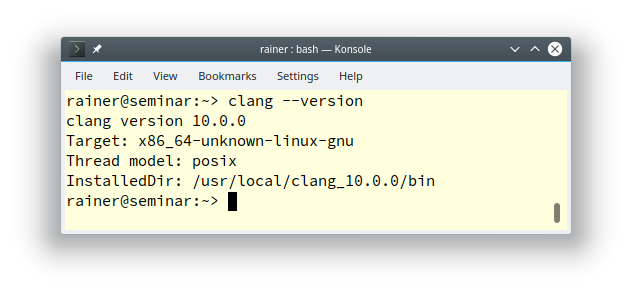
\includegraphics[width=0.8\textwidth]{content/3/chapter4/images/19.png}\\
Clang 10.0.0编译器
\end{center}

使用clang编译器,模块声明文件就是一个cpp文件。因此,我必须重新命名math.ixx文件为math.cpp。

\begin{lstlisting}[style=styleCXX]
// math.cpp

export module math;

export int add(int fir, int sec){
	return fir + sec;
}
\end{lstlisting}

客户端文件client.cpp没有改变,这是创建可执行文件的必要步骤。

\hspace*{\fill} \\ %插入空行
\noindent
\textbf{使用Clang编译器构建可执行文件}
\begin{tcblisting}{commandshell={}}
clang++ -std=c++2a -stdlib=libc++ -c math.cpp -Xclang -emit-module-interface \
   -o math.pcm

clang++ -std=c++2a -stdlib=libc++ -fprebuilt-module-path=. client.cpp math.pcm \
   -o client
\end{tcblisting}

\begin{itemize}
\item 
第1行创建模块math.pcm。后缀pcm代表预编译模块。标志-std=c++2a指定C++20标准的工作草案,-stdlib=libc++指定使用的C++标准库。标记组合-Xclang -emit-module-interface是创建预编译模块所必需的标志。

\item 
第4行创建可执行程序,使用模块math.pcm,并用-fprebuilt-module-path标志指定模块的路径。
\end{itemize}

\hspace*{\fill} \\ %插入空行
\noindent
\textbf{4.2.4.3\hspace{0.2cm}使用过的编译器}

我在这本书中使用的是Microsoft的cl.exe。Microsoft目前(2020年底)\href{https://en.cppreference.com/w/cpp/compiler_support}{对模块的最佳支持}的情况。Microsoft博客提供了两个很好的模块介绍:\href{https://docs.microsoft.com/en-us/cpp/cpp/modules-cpp?view=msvc-160&viewFallbackFrom=vs-2019}{概述C++模块}和\href{https://devblogs.microsoft.com/cppblog/c-modules-conformance-improvements-with-msvc-in-visual-studio-2019-16-5/}{C++模块的一致性改进与MSVC在Visual Studio 2019 16.5}。Clang和GCC都没有提供类似的介绍,因此在这些编译器中使用模块也非常困难。

\subsubsubsection{4.2.5\hspace{0.2cm}导出}

有三种方法可以导出模块接口单元中的名称。

\hspace*{\fill} \\ %插入空行
\noindent
\textbf{4.2.5.1\hspace{0.2cm}导出说明符}

可以显式地导出每个名称。

\begin{lstlisting}[style=styleCXX]
export module math;
export int mult(int fir, int sec);
export void doTheMath();
\end{lstlisting}

\hspace*{\fill} \\ %插入空行
\noindent
\textbf{4.2.5.2\hspace{0.2cm}导出组}

导出组会导出所有名称。

\begin{lstlisting}[style=styleCXX]
export module math;
export {
	int mult(int fir, int sec);
	void doTheMath();
}
\end{lstlisting}

\hspace*{\fill} \\ %插入空行
\noindent
\textbf{4.2.5.3\hspace{0.2cm}导出命名空间}

可以使用导出的命名空间,代替导出组。

\begin{lstlisting}[style=styleCXX]
export module math;
export namespace math {
	int mult(int fir, int sec);
	void doTheMath();
}
\end{lstlisting}

当客户端使用来自导出命名空间的名称时,必须限定这些名称。

只有没有内部链接的名称才可以导出。

\subsubsubsection{4.2.6\hspace{0.2cm}构造模块结构的指南}

来研究一下如何构造模块的指导方针。

\begin{lstlisting}[style=styleCXX]
module; // global module fragment
#include <headers for libraries not modularized so far>
export module math; // module declaration; starts the module purview
import <importing of other modules>
<non-exported declarations> // names only visibile inside the module
export namespace math {
	<exported declarations> // exported names
}
\end{lstlisting}

这个指导原则有一个目的:提供一个简化的模块结构,以及将要书写的内容。那么,这个模块结构有什么新东西呢?

\begin{itemize}
\item 
可选以关键字module开头的全局模块,之后和模块声明之前的位置,是包含头文件的正确位置。

\item 
模块声明导出模块math启动模块权限,该权限在翻译单元的末尾结束。

\item 
可以在模块权限的开始导入模块。导入的模块具有模块链接,在模块外部不可见。这一点也适用于非导出声明。

\item 
我将导出的名称放在命名空间math中,该名称与模块名称相同。

\item 
模块只有声明的名称。现在,一起来了解一下接口和模块的实现分离。
\end{itemize}

\subsubsubsection{4.2.7\hspace{0.2cm}模块接口单元和模块实现单元}

当模块变大时,应该将其组织成一个模块接口单元和一个或多个模块实现单元。按照前面提到的构造模块的指导原则,我将重构math模块。

\hspace*{\fill} \\ %插入空行
\noindent
\textbf{4.2.7.1\hspace{0.2cm}模块接口单元}

\begin{lstlisting}[style=styleCXX]
// mathInterfaceUnit.ixx

module;

#include <vector>

export module math;

export namespace math {

	int add(int fir, int sec);
	
	int getProduct(const std::vector<int>& vec);

}
\end{lstlisting}

\begin{itemize}
\item 
模块接口单元包含导出模块声明:export module math(第7行)。

\item 
导出add和getProduct(第11和13行)。

\item 
一个模块只能有一个模块接口单元。
\end{itemize}

\hspace*{\fill} \\ %插入空行
\noindent
\textbf{4.2.7.2\hspace{0.2cm}模块的实现单元}

\begin{lstlisting}[style=styleCXX]
// mathImplementationUnit.cpp

module math;

#include <numeric>

namespace math {

	int add(int fir, int sec) {
		return fir + sec;
	}
	
	int getProduct(const std::vector<int>& vec) {
		return std::accumulate(vec.begin(), vec.end(), 1, std::multiplies<int>());
	}
}
\end{lstlisting}

\begin{itemize}
\item 
模块实现单元包含非导出模块声明:module math;(第3行)。

\item 
一个模块可以有多个模块实现单元。
\end{itemize}

\hspace*{\fill} \\ %插入空行
\noindent
\textbf{4.2.7.3\hspace{0.2cm}主程序}

\begin{lstlisting}[style=styleCXX]
// client3.cpp

#include <iostream>
#include <vector>

import math;

int main() {

	std::cout << '\n';
	
	std::cout << "math::add(2000, 20): " << math::add(2000, 20) << '\n';
	
	std::vector<int> myVec{1, 2, 3, 4, 5, 6, 7, 8, 9, 10};
	
	std::cout << "math::getProduct(myVec): " << math::getProduct(myVec) << '\n';
	
	std::cout << '\n';

}
\end{lstlisting}

从用户的角度来看,除了导入模块math(第6行),还需要添加命名空间math。

解释依赖于编译器,我把它们放在一个单独的提示框中。若各位想尝试一下,这些信息还是有参考意义的。


\begin{tcolorbox}[breakable,enhanced jigsaw,colback=blue!5!white,colframe=blue!75!black,title={使用Microsoft编译器构建可执行文件}]
	
手动构建可执行文件包括以下几个步骤。

\hspace*{\fill} \\ %插入空行
\noindent
\textbf{用模块接口单元和模块实现单元构建模块}
\begin{tcblisting}{commandshell={}}
cl.exe /c /experimental:module mathInterfaceUnit.ixx /EHsc
cl.exe /c /experimental:module mathImplementationUnit.cpp /EHsc
cl.exe /c /experimental:module client3.cpp /EHsc
cl.exe client3.obj mathInterfaceUnit.obj mathImplementationUnit.obj
\end{tcblisting}

\begin{itemize}
\item 
第1行:创建了对象文件mathInterfaceUnit.obj和模块接口文件math.ifc。

\item 
第2行:创建了对象文件mathImplementationUnit.obj。

\item 
第3行:创建对象文件client3.obj。

\item 
第4行:创建可执行文件client3.exe。
\end{itemize}

对于Microsoft编译器,必须指定异常处理模型(/EHsc),并启用模块支持:/experimental:module。

最后,是程序的输出:

\begin{center}
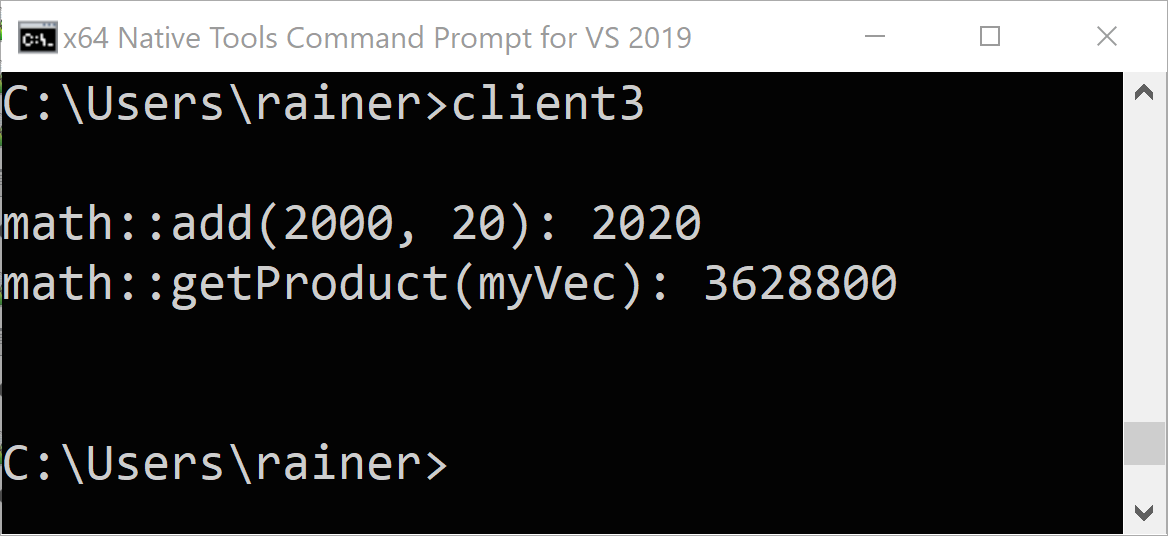
\includegraphics[width=0.6\textwidth]{content/3/chapter4/images/20.png}\\
执行程序client2.exe
\end{center}
\end{tcolorbox}

\subsubsubsection{4.2.8\hspace{0.2cm}子模块和模块分区}

当模块变大时,希望将其功能划分为可管理的组件。C++20模块提供了两种方法:子模块和分区。

\hspace*{\fill} \\ %插入空行
\noindent
\textbf{4.2.8.1\hspace{0.2cm}子模块}

模块可以导入模块,然后重新导出它们。

下面的例子中,math模块导入了子模块math.math1和math.math2。

\begin{lstlisting}[style=styleCXX]
// mathModule.ixx
export module math;
export import math.math1;
export import math.math2;
\end{lstlisting}

表达式export import math.math1将math.math1导入math模块。并将其作为math模块的一部分重新导出。

完整起见,下面是完整的math.math1和math.math2。我使用单独的代码段,将math模块与其子模块分开。实际开发中,代码没必要分开。

\hspace*{\fill} \\ %插入空行
\noindent
\textbf{子模块math.math1}
\begin{lstlisting}[style=styleCXX]
// mathModule1.ixx
export module math.math1;
export int add(int fir, int sec) {
	return fir + sec;
}
\end{lstlisting}

\noindent
\textbf{子模块math.math2}
\begin{lstlisting}[style=styleCXX]
// mathModule2.ixx
export module math.math2;
export {
	int mul(int fir, int sec) {
		return fir * sec;
	}
}
\end{lstlisting}

仔细观察,会发现math模块中的export语句相较之前有所不同。math.math1使用导出说明符,而math.math2则使用导出组或导出块。

从使用者的角度来看,使用math模块非常简单。

\hspace*{\fill} \\ %插入空行
\noindent
\textbf{主程序}
\begin{lstlisting}[style=styleCXX]
// mathModuleClient.cpp
#include <iostream>
import math;
int main() {
	std::cout << '\n';
	std::cout << "add(3, 4): " << add(3, 4) << '\n';
	std::cout << "mul(3, 4): " << mul(3, 4) << '\n';
}
\end{lstlisting}

编译和执行程序可以得到预期输出。

\begin{center}
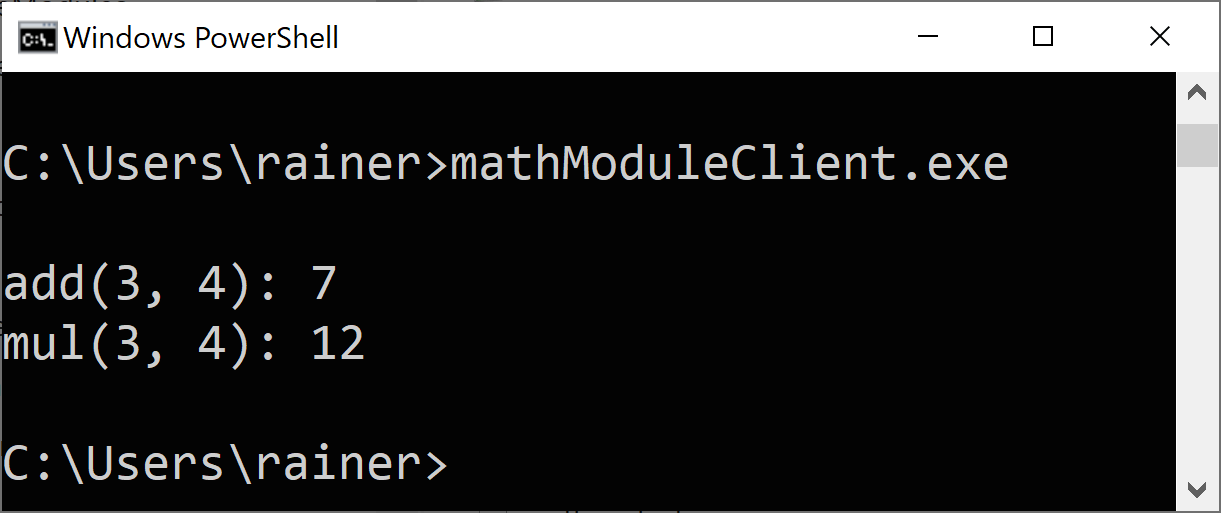
\includegraphics[width=0.6\textwidth]{content/3/chapter4/images/21.png}\\
模块和子模块的用法
\end{center}

\begin{tcolorbox}[breakable,enhanced jigsaw,colback=blue!5!white,colframe=blue!75!black,title={使用Microsoft编译器构建可执行文件}]
	
模块和其子模块如何一同构建可执行文件

\begin{tcblisting}{commandshell={}}
cl.exe /c /experimental:module mathModule1.ixx /EHsc
cl.exe /c /experimental:module mathModule2.ixx /EHsc
cl.exe /c /experimental:module mathModule.ixx /EHsc
cl.exe /EHsc /experimental:module mathModuleClient.cpp \
  mathModule1.obj mathModule2.obj mathModule.obj
\end{tcblisting}

这三个模块的每个编译过程都会创建两个工件:IFC文件(接口文件)*.ifc在最后一行隐式使用,*.obj文件在最后一行显式使用。

\end{tcolorbox}

子模块其实也是模块,每个子模块都有一个模块声明。因此,用户可以只使用其中之一,所以创建一个只使用math.math1模块的主程序。

\hspace*{\fill} \\ %插入空行
\noindent
主程序只使用子模块math.math1
\begin{lstlisting}[style=styleCXX]
// mathModuleClient1.cpp
#include <iostream>
import math.math1;
int main() {
	std::cout << '\n';
	std::cout << "add(3, 4): " << add(3, 4) << '\n';
}
\end{lstlisting}

\begin{center}
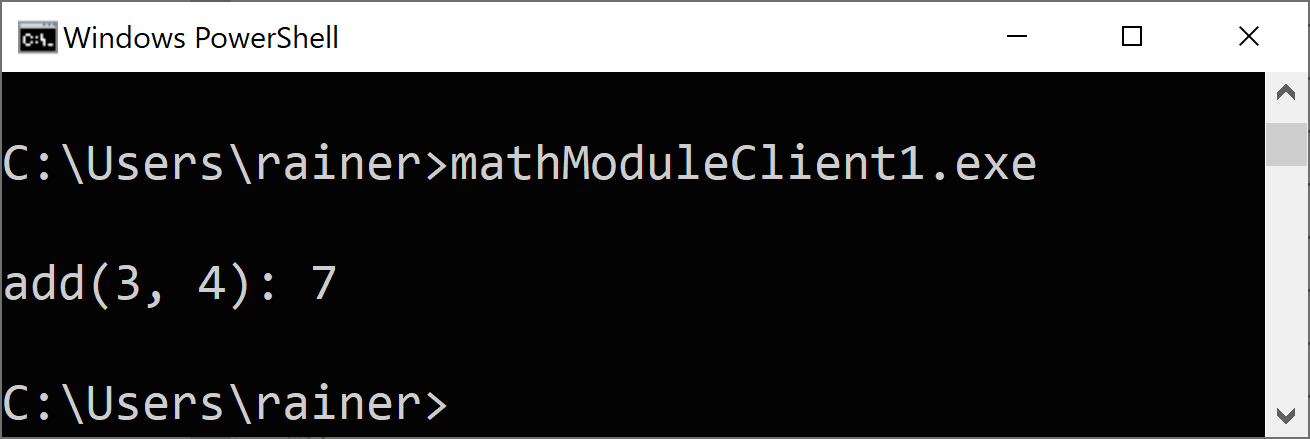
\includegraphics[width=0.6\textwidth]{content/3/chapter4/images/22.png}\\
子模块和模块的用法
\end{center}

将模块划分为模块和子模块,是模块设计者让模块的用户可以导入模块的细粒度部分的一种方法。不过,这个观察结果不适用于模块分区。

\hspace*{\fill} \\ %插入空行
\noindent
\textbf{4.2.8.2\hspace{0.2cm}模块分区}

A module can be divided into partitions. Each partition consists of a module interface unit (partition interface file) and zero or more module implementation units (see Module Interface Unit and Module Implementation Unit). The names that the partitions export are imported and re-exported by the primary module interface unit (primary interface file). The names of a partition must begin with the name of the module. The partitions cannot exist on their own.

The description of module partitions is more difficult to understand than its implementation. In the following lines, I rewrite the math module and its submodules math.math1 and math.math2 (see Submodules) to module partitions. In this straightforward process, I refer to the shortly introduced terms of module partitions.

\hspace*{\fill} \\ %插入空行
\noindent
Primary interface file
\begin{lstlisting}[style=styleCXX]
// mathPartition.ixx

export module math;

export import :math1;
export import :math2;
\end{lstlisting}

The primary interface file consists of the module declaration (line 3). It imports and re-exports the partitions math1 and math2 using colons (lines 5 and 6). The name of the partitions must begin with the name of the module. Consequently, you don’t have to specify them.

\hspace*{\fill} \\ %插入空行
\noindent
First module partition
\begin{lstlisting}[style=styleCXX]
// mathPartition1.ixx

export module math:math1;

export int add(int fir, int sec) {
	return fir + sec;
}
\end{lstlisting}

\hspace*{\fill} \\ %插入空行
\noindent
Second module partition
\begin{lstlisting}[style=styleCXX]
// mathPartition2.ixx

export module math:math2;

export {
	int mul(int fir, int sec) {
		return fir * sec;
	}
}
\end{lstlisting}

Similar to the module declaration, the expressions export module math:math1 and export module math:math2 (line 3) declare a module interface partition. A module interface partition is also a module interface unit. The name math stands for the module and the names math1 or math2 for the partition.

\hspace*{\fill} \\ %插入空行
\noindent
Import the module partition
\begin{lstlisting}[style=styleCXX]
// mathModuleClient.cpp
import math;
int main() {
	std::cout << '\n';
	std::cout << "add(3, 4): " << add(3, 4) << '\n';
	std::cout << "mul(3, 4): " << mul(3, 4) << '\n';
}
\end{lstlisting}

You may have already assumed it: The client program is identical to the client program I previously used with submodules. The same observation holds for the creation of the executable and the execution of the program:

\begin{center}
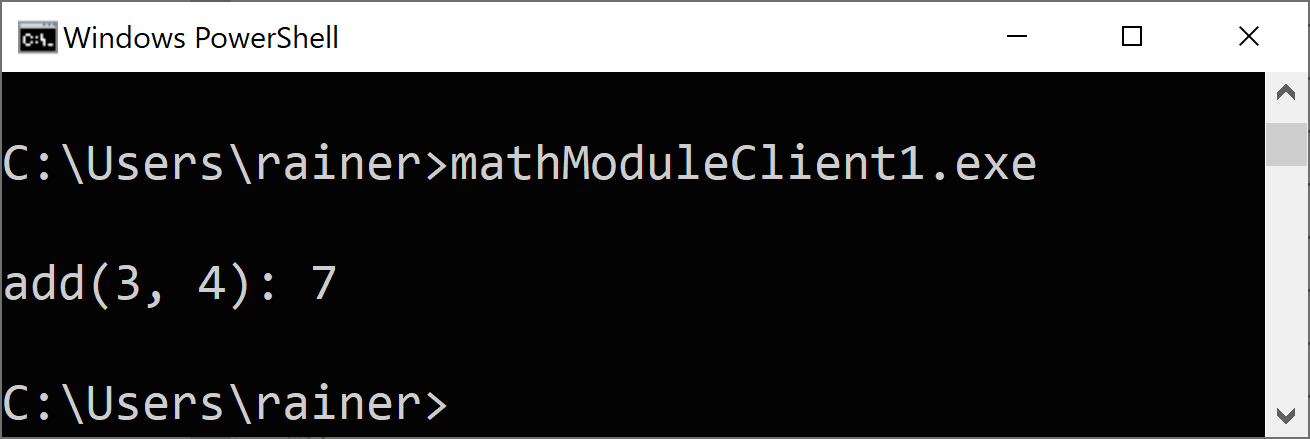
\includegraphics[width=0.6\textwidth]{content/3/chapter4/images/23.png}\\
The usage of function modules and submodules
\end{center}

\subsubsubsection{4.2.9\hspace{0.2cm} Templates in Modules}

I often hear the question: How are templates exported by modules? When you instantiate a template, its definition must be available. This is the reason that template definitions are hosted in headers. Conceptually, the usage of a template has the following structure

\hspace*{\fill} \\ %插入空行
\noindent
4.2.9.1\hspace{0.2cm} Without Modules

\begin{itemize}
\item 
templateSum.h

\noindent
Definition of the function template sum
\begin{lstlisting}[style=styleCXX]
// templateSum.h
template <typename T, typename T2>
auto sum(T fir, T2 sec) {
	return fir + sec;
}
\end{lstlisting}

\item 
sumMain.cpp

\noindent
Use of the template sum
\begin{lstlisting}[style=styleCXX]
// sumMain.cpp
#include <templateSum.h>
int main() {
	sum(1, 1.5);
}
\end{lstlisting}
\end{itemize}

The main program directly includes the header templateSum.h. The call sum(1, 1.5) triggers the template instantiation. In this case, the compiler generates out of the function template sum the concrete function sum, which takes an int and a double as arguments. If you want to visualize this process, use the example on \href{https://cppinsights.io/}{C++ Insights}.

\hspace*{\fill} \\ %插入空行
\noindent
4.2.9.2\hspace{0.2cm} With Modules

With C++20, templates can and should be in modules. Modules have a unique internal representation that is neither source code nor assembly. This representation is a kind of an \href{https://en.wikipedia.org/wiki/Abstract_syntax_tree}{abstract syntax tree} (AST). Thanks to this AST, the template definition is available during template instantiation.

In the following example, I define the function template sum in module math.

\begin{itemize}
\item 
mathModuleTemplate.ixx

\noindent
Definition of the function template sum
\begin{lstlisting}[style=styleCXX]
// mathModuleTemplate.ixx
export module math;
export namespace math {
	template <typename T, typename T2>
	auto sum(T fir, T2 sec) {
		return fir + sec;
	}
}
\end{lstlisting}

\item 
clientTemplate.cpp

\noindent
Use of the function template sum
\begin{lstlisting}[style=styleCXX]
// clientTemplate.cpp
#include <iostream>
import math;
int main() {
	std::cout << '\n';
	std::cout << "math::sum(2000, 11): " << math::sum(2000, 11) << '\n';
	std::cout << "math::sum(2013.5, 0.5): " << math::sum(2013.5, 0.5) << '\n';
	std::cout << "math::sum(2017, false): " << math::sum(2017, false) << '\n';
}
\end{lstlisting}
\end{itemize}

The command line to compile the program is not different from the previous ones. Consequently, I skip it and present the output of the program directly:

\begin{center}
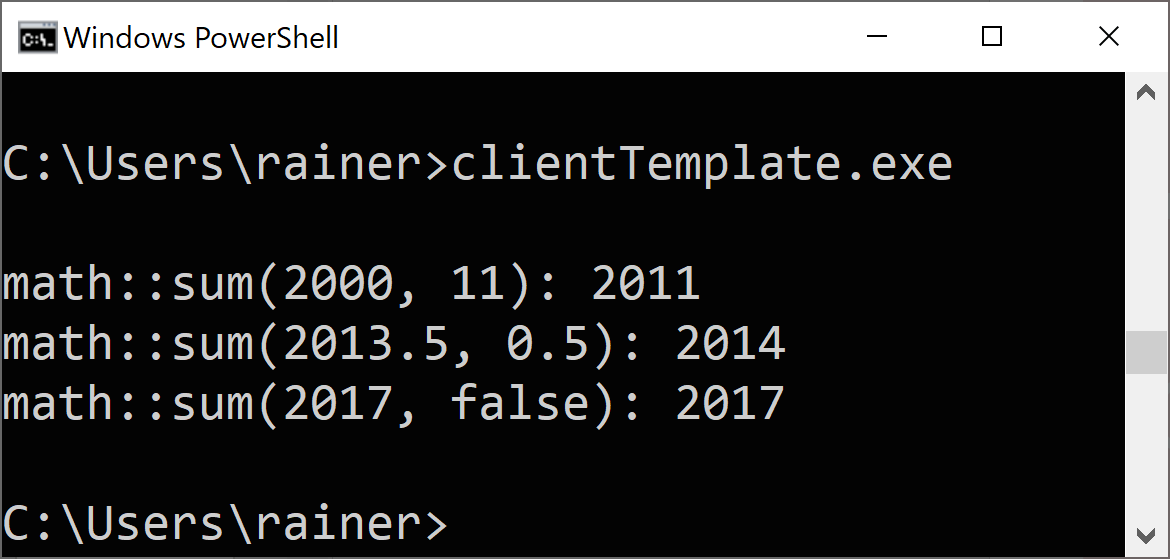
\includegraphics[width=0.6\textwidth]{content/3/chapter4/images/24.png}\\
Use of the function template sum
\end{center}

With modules, we get a new kind of linkage.

\subsubsubsection{4.2.10\hspace{0.2cm} Module Linkage}

Until C++20, C++ supported two kinds of linkage: internal linkage and external linkage.

\begin{itemize}
\item 
Internal linkage: Names with internal linkage are not accessible outside the translation unit. Internal linkage includes mainly namespace-scope names that are declared static and members of anonymous namespaces.

\item 
Internal linkage: Names with internal linkage are not accessible outside the translation unit. Internal linkage includes mainly namespace-scope names that are declared static and members of anonymous namespaces.
\end{itemize}

Modules introduce module linkage:

\begin{itemize}
\item 
Module linkage: Names with module linkage are only accessible inside the module. Names have module linkage if they don’t have external linkage and they are not exported.
\end{itemize}

A small variation of the previous module declaration mathModuleTemplate.ixx makes my point. Imagine that I want to return to the user of my function template sum not only the result of the addition, but also the return type the compiler deduces.

\hspace*{\fill} \\ %插入空行
\noindent
An improved definition of the function template sum
\begin{lstlisting}[style=styleCXX]
// mathModuleTemplate1.ixx

module;

#include <iostream>
#include <typeinfo>
#include <utility>

export module math;

emplate <typename T>
auto showType(T&& t) {
	return typeid(std::forward<T>(t)).name();
}

export namespace math {

	template <typename T, typename T2>
	auto sum(T fir, T2 sec) {
		auto res = fir + sec;
		return std::make_pair(res, showType(res));
	}

}
\end{lstlisting}

nstead of the sum of the numbers, the function template sum returns a \href{https://en.cppreference.com/w/cpp/utility/pair}{std::pair} (line 21) consisting of the sum and a string representation of the type of the value res. Note that I put the function template showType (line 11) outside the exported namespace math (line 16). Consequently, invoking it from outside the module math is not possible. Function template showType uses \href{https://www.modernescpp.com/index.php/perfect-forwarding}{perfect forwarding} to preserve the value categories of the function argument t. The \href{https://en.cppreference.com/w/cpp/language/typeid}{typeid} operator queries information about the type at run time (\href{https://en.cppreference.com/w/cpp/types}{run time type identification (RTTI)}).

\hspace*{\fill} \\ %插入空行
\noindent
Use of the improved function template sum
\begin{lstlisting}[style=styleCXX]
// clientTemplate1.cpp

#include <iostream>
import math;

int main() {
	
	std::cout << '\n';
	
	auto [val, message] = math::sum(2000, 11);
	std::cout << "math::sum(2000, 11): " << val << "; type: " << message << '\n';
	
	auto [val1, message1] = math::sum(2013.5, 0.5);
	std::cout << "math::sum(2013.5, 0.5): " << val1 << "; type: " << message1
			  << '\n';
	auto [val2, message2] = math::sum(2017, false);
	std::cout << "math::sum(2017, false): " << val2 << "; type: " << message2
			  << '\n';

}
\end{lstlisting}

Now, the program displays the value of the summation and a string representation of the automatically deduced type.

\begin{center}
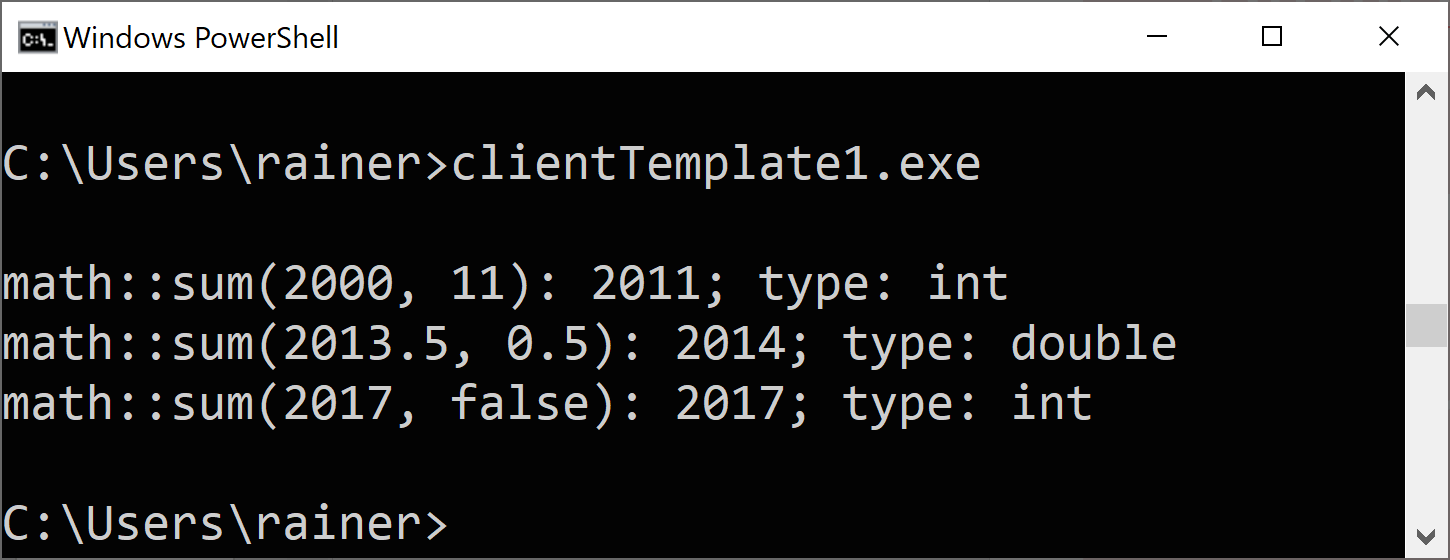
\includegraphics[width=0.8\textwidth]{content/3/chapter4/images/25.png}\\
Use of the improved function template sum
\end{center}

\subsubsubsection{4.2.11\hspace{0.2cm} Header Units}

At the end of 2020, no compiler, so far, supports header units. Header units are a smooth way to transition from headers to modules. You just have to replace the \#include directive with the new import directive.

\hspace*{\fill} \\ %插入空行
\noindent
Replacing \#include directives with import directives
\begin{lstlisting}[style=styleCXX]
#include <vector> => import <vector>;
#include "myHeader.h" => import "myHeader.h";
\end{lstlisting}

First, import respects the same lookup rules as include. This means in the case of the quotes ("myHeader.h") that the lookup first searches in the local directory before it continues with the system search path.

Second, this is way more than text replacement. In this case, the compiler generates something module-like out of the import directive and treats the result as if it would be a module. The importing module statement gets all exportable names from the header. The exported names include macros. Importing these synthesized header units is faster than including header files and comparable in speed to precompiled headers.

\hspace*{\fill} \\ %插入空行
\noindent
4.2.11.1\hspace{0.2cm} One Drawback

There is one drawback with header units. Not all headers are importable. Which headers are importable is \href{https://en.cppreference.com/w/cpp/language/ub}{implementation-defined}, but the C++ standard guarantees that all standard library headers are importable headers. The ability to import excludes C headers. They are just wrapped in the std namespace. For example <cstring> is the C++ wrapper for <string.h>. You can easily identify the wrapped C header because the pattern is: xxx.h gets cxxx.

\begin{tcolorbox}[colback=mygreen!5!white,colframe=mygreen!75!black,title=Building the Executable with the Microsoft Compiler]

\begin{itemize}
\item 
Modules overcome the deficiencies of headers and macros, in particular. Their import is literally for free, and in contrast to macros, the sequence in which you import does not matter. Additionally, they overcome name collisions.

\item 
A module consists of a module interface unit and a module implementation unit. There must be one module interface unit having the exporting module declaration and arbitrarily many module implementation units. Names that are not exported in the module interface have module linkage and cannot be used outside the module.

\item 
Modules can have headers or import and re-export other modules.

\item 
The standard library in C++20 is not modularized. Building your modules is with C++20 a challenging task.

\item 
To structure large software systems, modules provide two ways: submodules and partitions. In contrast to a partition, a submodule can live on its own.

\item 
Thanks to header units, you can replace an include statement with an import statement, and the compiler autogenerates a module.
\end{itemize}

\end{tcolorbox}











































